\documentclass[12pt,letterpaper]{article}

\usepackage{hyperref}

\usepackage{amsmath}
\usepackage{amssymb}
\usepackage{amsthm}

\usepackage{cleveref}

\usepackage{algorithm}
\usepackage{algpseudocode}
\usepackage{xcolor}
\usepackage{tikz}
\usepackage{tikz-cd}
\usepackage{float}

\newcommand*{\bigo}{\mathcal{O}}
\newcommand*{\R}{\mathbb{R}}
\newtheorem{theorem}{theorem}[section]
\newtheorem{definition}[theorem]{Definition}
\newtheorem{lemma}[theorem]{Lemma}
\newtheorem{corollary}[theorem]{Corollary}
\newtheorem{observation}[theorem]{Observation}

\setlength\parindent{0pt}

\title{Computing the convex hull of solution vectors to the airplane refueling problem to find a general description}
\author{Zixuan Fan}

\begin{document}
\maketitle

\section{Motivation}

\subsection{Problem Statement}
The Airplane Refueling Problem is a combinatorial problem that is 
neither known to be NP-complete nor polynomially solvable. 
It reflects a real-life problem, where a fleet of airplanes refuels each other 
to maximize the flying distance. Formally, we give the following definition. 
\begin{definition}
 Given $n$ planes each with a tank $w_j$ and consumption rate $p_j$,
 what is the longest time/distance that this fleet of planes can fly with full tanks,
 if they can refuel each other?
\end{definition}
An intuitive idea is consuming the tank of only one plane 
at a time, and dropping it out after its tank is empty. This approach 
finds a \textit{drop out ordering} $\sigma$
that maximizes the objective function 
\begin{align*}
    \max \sum_{j=1}^{n} \dfrac{w_{\sigma(j)}}{\sum_{k = j}^n p_{\sigma(k)}}
\end{align*}
To elaborate on this objective function, only the planes with indexing no less than $j$ in order $\sigma$
are consuming the tank of the $j$-th plane. Thus, the time until the $j$-th plane is fully consumed is 
\begin{align*}
    \dfrac{w_{\sigma(j)}}{\sum_{k = j}^n p_{\sigma(k)}}
\end{align*}
while the sum of all these times is the objective maximization function.

\subsection{Scheduling and Mathematical Programming}
Based on understaning mentioned above, Woeginger et al. formalized this problem as a scheduling problem. \cite{woeginger2010scheduling}
In the scheduling context, we view $\sigma$ as permutation $\pi$, the reverse of ordering.
We can also change the objective function to a simpler form. 
\begin{align*}
    \sum_{j=1}^{n} \dfrac{w_{\sigma(j)}}{\sum_{k = j}^n p_{\sigma(k)}} = \sum_{j = 1}^n \dfrac{w_{\pi(j)}}{\sum_{k = 1}^j p_{\pi(k)}}
\end{align*}
where $p$ stands for the processing time of the $j$-th job now. 
For simplicity, we also introduce the completion time $C_j$
that is, 
the time until the $j$-th plane is consumed.
\begin{align*}
    \sum_{j = 1}^n \dfrac{w_{\pi(j)}}{\sum_{k = 1}^j p_{\pi(k)}} =  \sum_{j = 1}^n \dfrac{w_{j}}{C_j}
\end{align*}
With all premises explained, we can also introduce a mathematical programming formulation. Note that $S_n$ stands for the permutation group of order $n$. 
\begin{align}
    &\max \sum_{j = 1}^n \dfrac{w_j}{C_j} \label{eq:mathprog} \tag{A} \\ 
    \text{s. t.\ }& C_{\pi(j+1)} - C_{\pi(j)} = p_{\pi(j)} \forall j \nonumber \\
    & \pi \in S_n \nonumber
\end{align}
Should this be a linear program, we can solve it in polynomial time. However, the objective function 
itself is not linear, while the constraints involving permutation are also complicated. 
Hence, we want to explore the different possibilities for solving this problem concerning mathematical programming. 

\section{Theoretical Backgrounds}
The fundamental idea is reformulating the problem as a linear program or a convex program, which 
is solvable in polynomial time. By removing the completion time in \ref{eq:mathprog}, we obtain a
linear objective function. 
\begin{align*}
    &\max w^T \cdot x \label{eq:linobj} \tag{B} \\ 
    \text{s. t.\ }& C_{\pi(j+1)} - C_{\pi(j)} = p_{\pi(j)} \forall j \\
    & \pi \text{ is a permutation} \\ 
    & x_j = \dfrac{1}{C_j} \ \ \forall j \in [n] 
\end{align*}
Following this formulation, an intuition is
computing the convex hull of feasible solutions, which are all possible combinations of the completion time's reciprocals. 
\begin{align*}
 s = \left( \dfrac{1}{C_1}, \dfrac{1}{C_2}, ..., \dfrac{1}{C_n}\right)
\end{align*} 
We can observe that each solution vector corresponds to a permutation of the consumption rate. 
More precisely, the longer the completion time, the later the tank is consumed in the permutation.
There are $n!$ many of these vectors, and the convex hull is a polytope in $\R^n$. 
Thus, we are interested in a special shape, a permutahedron.

\subsection{Permutation Matrices}
Before we take a closer look at permutahedra, we need to introduce permutation matrices.
\begin{definition}
    A permutation matrix $M \in \R^{n \times n}$ is a square binary matrix describing a permutation $\pi$.
    For each entry $m_{ij}$ of $M$, the following constraints must hold.
    \begin{enumerate}
        \item $m_{ij} \in \{0, 1\}$ for all $i, j$
        \item $\sum_{i = 1}^n m_{ij} = 1$, for all $j$
        \item $\sum_{j = 1}^n m_{ij} = 1$, for all $i$
    \end{enumerate}
\end{definition}
First, we show that there is a bijective relationship between permutation matrices and permutations, i.e. permutation matrices 
can be used to describe permutations.
\begin{lemma}
    There is a bijective mapping between permutation matrices and permutations.
\end{lemma}
\begin{proof}
    For each permutation $\pi \in S_n$, we construct a permutation matrix $M$.
    \begin{align*}
        m_{ij} = 
        \begin{cases}
            1 & \text{if } \pi(j) = i \\
            0 & \text{otherwise}
        \end{cases}
    \end{align*}
\end{proof}
A property of permutation matrices is that they are doubly stochastic, i.e., the sum of each row and each column is 1.
In the special case of permutation matrices, the matrix is also orthogonal.
\begin{lemma}
    If $M$ is a permutation matrix, then $M$ is orthogonal.
\end{lemma}
\begin{proof}
    We consider the matrix product $MM^T$. It suffices to show $MM^T = I$. The $(i, j)$-th entry of $MM^T$ is given by 
    \begin{align*}
        (MM^T)_{ij} = \sum_{k = 1}^n m_{ik}m_{jk}
    \end{align*}
    If $i \neq j$, then we are summing up the product of entries in two different rows. 
    Since there is only one entry equal to one in each column, the products are all zero. Hence, their sum is also zero. \\ 
    If $i \neq j$, then we are summing up the product of entries in the same row.
    There is only one entry equal to one in each row, so the product is one. \\
    In conclusion, the matrix product is the identity matrix, and $M$ is orthogonal.
\end{proof}
\begin{corollary}
    \label{cor:inverse}
    If $M$ is a permutation matrix, then $M^{-1} = M^T$.
\end{corollary}


\subsection{Permutahedron}
A permutahedron is a polytope that is the convex hull of all vertices representing a permutation i.e. $\{(\pi(1), \pi(2), \cdots, \pi(k) | \pi \in S_n) \}$. \cite{doi:10.1137/0122054}
In the permutahedron of the $n$-th order $P_n$, each vertex is a permutation of $n$ elements.
Hence, there are $n!$ many vertices in $P_n$. For example, a hexagon is a second-order permutahedron. 
First, we take a look at a simple LP formulation of permutahedra. 
\begin{align*}
    \sum_{i \in S} x_i = \sum_{k = n - |S| + 1}^n k, \ \ \forall \emptyset \neq S \subset [n]
\end{align*}
We need $2^n - 2$ facets to define the polytope.
\\
Although the number of faces is not polynomial in $n$,
some symmetric properties were discovered and are useful for optimization. Some researchers\textbf{cite later}
have found an extended formulation $\R^{k^2+k} \rightarrow \R^{k}$, which allows us 
to solve the LP on $P_k$ in polynomial time. 

\begin{align}
    &\sum_{j \in [n]} y_{ij} = 1, \ \ \forall i \in [n], \sum_{i \in [n]} y_{ij} = 1, \ \ \forall j \in[n] \label{eq:C} \tag{C} \\ 
    &y_{ij} \geq 0, \ \ \forall i, j \in [n] \nonumber 
\end{align}
The trick is the permutation matrix. We show that this is a formulation of the 
convex hull of all permutation metrices.
\begin{lemma}
    The polytope defined by \ref{eq:C} is the convex hull of all permutation matrices to order $n$.
\end{lemma}
\begin{proof}
    It suffices to show that \ref{eq:C} describes the set of all convex combinations of permutation matrices. \\
    $\impliedby$: Let $M^1, M^2, \cdots M^k$ be arbitrary distinct permutation matrices. Let $\lambda_1, \lambda_2, \cdots \lambda_k \in [0, 1]$ be arbitrary
    such that $\sum_{i=1}^k = 1$.
    We obtain a convex combination $Y = \sum_{l = 0}^k \lambda_l M^i$.We check each constraints accordingly. 
    \begin{align*}
    \sum_{j \in [n]} y_{ij} &= \sum_{j \in [n]} \sum_{l = 0}^k \lambda_l m_{ij}^l \\
    &= \sum_{l = 0}^k \lambda_l \sum_{j \in [n]} m_{ij} = \sum_{l = 0}^k \lambda_l = 1 \\ 
    \sum_{i \in [n]} y_{ij} &= \sum_{i \in [n]} \sum_{l = 0}^k \lambda_l m_{ij}^l \\
    &= \sum_{l = 0}^k \lambda_l \sum_{i \in [n]} m_{ij} = \sum_{l = 0}^k \lambda_l = 1 \\ 
    y_{ij} &= \sum_{l = 0}^k \lambda_k m_{ij}^l \geq \sum_{l = 0}^k \lambda_k \cdot 0  = 0 
    \end{align*}
    We may conclude that $Y$ is in the polytope described by \ref{eq:C}. \\
    $\implies$: Let $Y$ be a feasible solution to constraints in \ref{eq:C}. 
    We observe that $Y$ is doubly stochastic. It is shown by Birkhoff's theorem \textbf{cite Birkhoff} that 
    $Y$ is a convex combination of permutation matrices. 
\end{proof}

As a consequence, we can obtain the vertices representing the permutations by 
\begin{align*}
    x_i = \sum_{j = 0}^n j \cdot y_{ij} \forall i \in[n]
\end{align*}
In this way, we are able to reduce the number of constraints to $n^2 + 3n$ under $R^{n^2 + n}$.
This extended formulation is helpful in terms of both linear programming and non-linear programming. 

\section{Attempts with non-linear programming}
Inspired by the permutahedron, we want to find a similar formulation for the polytope of the completion time,
because there is a permutation-related structure in the polytope. 

\subsection{Formulation}
Recall in \ref{eq:linobj}, the completion time $C_j$ is 
an acculumating sum of the processing time $p_j$ with regard to 
permutation $\pi$. We would exploit the formulation in \ref{eq:C} 
to find a similar formulation for the completion time. The figure \ref{fig:completion}
shows how the completion time is constructed with a permutation, and respectively with a permutation matrix.
\begin{figure}[h!]
    \centering
    \begin{tikzcd}
        \begin{pmatrix}
            p_1 \\ 
            \vdots \\
            p_n
        \end{pmatrix} 
        \arrow[r, "\pi"]
        & \begin{pmatrix}
            p_{\pi(1)} \\ 
            \vdots \\
            p_{\pi(n)}
        \end{pmatrix}
        \arrow[r, "sum"]
        & \begin{pmatrix}
            p_{\pi(1)} \\ 
            \vdots \\
            \sum_{i = 0}^n p_{\pi(i)}
        \end{pmatrix} = 
        \begin{pmatrix}
            C_{\pi(1)} \\
            \vdots  \\
            C_{\pi(n)}
        \end{pmatrix}
        \arrow[r, "\pi^{-1}"]
        & \begin{pmatrix}
            C_1 \\ 
            \vdots \\
            C_n
        \end{pmatrix}
    \end{tikzcd}
    \caption{Construction of completion time}
    \label{fig:completion}
\end{figure}
Apparently, such operations can be formulated with matrices. 
We introduce a matrix $S$ for the summation operation. $S$ is a lower-triangular matrix with all ones.
In addition, we retain the permutation matrix as shown in \ref{eq:C}.
For naming conventions of variables, we use $y_i$ for completion and $z_i$ for permutation matrices 
in the following formulation.
\begin{align*}
    \max w^Tx& \text{ s.t. } \label{eq:D} \tag{D} \\
 x_i y_i &= 1 \ \forall i, \ \ y \geq 0, \\ 
    \sum_{i \in [n]} z_{ij} &= 1 \forall j,  \ \ 
    \sum_{j \in [n]} z_{ij} = 1 \forall i,  \ z_{ij} \in \{0, 1\} \forall i, j \\ 
    \Pi &= (z_{ij}), S = \begin{pmatrix}
        1 & \cdots & 0 \\ 
        \cdots & \cdots & \cdots \\ 
        1 & \cdots & 1
    \end{pmatrix} \\
 y &= \Pi^T S \Pi p 
\end{align*}
One special part of the formulation is $\Pi^T$, where the transpose 
of the permutation matrix is used. This stems from the result in \ref{cor:inverse},
where the inverse of a permutation matrix is its transpose.

\subsection{Convexity}
Now that we have a correct formulation, we are ready to implement and execute some experiments.
However, the given formulation serves as a mixed-integer nonlinear program. 
For actual execution, we have first convert it into a non-integer program, and check its convexity afterwards.
In a classical manner, the binary integer variables are relaxed to continuous variables.
\begin{align*}
 z_{ij} \in [0, 1] \ \forall i, j
\end{align*}
There are also quadratic equality constraints, where we lose the convexity for the equal relation. 
There are roundabouts to make them convex, by introducing inequalities. 
\begin{align*}
 x_i y_i &\geq 1 \ \forall i \\
 y &\geq \Pi^T S \Pi p
\end{align*}
In this way, we can obtain a feasible, convex, but unbounded area. 
Unboundedness is another problem, for we are doing a maximization. 
Unfortunately, we cannot solve the problem with this non-linear programming approach. 
\textbf{DO I HAVE TO SHOW THE CONVEXITY HERE?}

\subsection{Simple Practical Experiments}
Although the program is not convex, we can still run it in some scientific computing software.
For software based on Disciplined Convex Programming, like CVXPY \cite{diamond2016cvxpy}, we cannot even run the program 
because it has semantic checks on convexity. For software that does not require this check, like SCIP \cite{BolusaniEtal2024ZR}, the program 
ends up in a dead loop without termination. 

\section{Attempts with linear programming}
Since finding a convex formulation directly from permutahedra is impossible, 
we wonder if we can find the polytope describing the solution vectors in a linear programming way.
Without too many theoretical backgrounds, we decided to do some practical computation on those vertices.

\paragraph{Input Generation}
As we have analyzed in the first attempt, we want to compute the polytope of all solution vectors 
\begin{align*}
 s = \left( \dfrac{1}{C_1}, \dfrac{1}{C_2}, ..., \dfrac{1}{C_n} \right)
\end{align*}
Since the completion time is based on the permutation $\pi$, we need a few steps to generate all possible 
vectors. 
\begin{enumerate}
    \item Generate a randomized/special consumption time $p_j$
    \item Pick a permutation $\pi$, arrange the consumption time in the order of $\pi$
    \item Compute the completion time by $C_1 = p_1$ and $C_{i+1} = C_i + p_{i+1}$
    \item Compute the inverse of $C_j$
    \item Repeat until all permutations are visited
\end{enumerate}
This results in $n!$ vertices in $\R^n$. A straightforward traversal on the vertices is not 
polynomial-time, but it may help us to find some polynomial-time structure within the polytope.

\paragraph{Setups}
For the computation of the polytope with vertices, we use the scientific computing software polymake \cite{assarf2017computing}.
Polymake is a software that can compute the convex hull of a set of points in $\R^n$. 
The computation was run on a private computer with Intel i5-12600k CPU with 16 GB RAM. 

\subsection{First Computation}
Although the computation of the polytope is polynomial-time in the number of vertices, our computation takes 
a significant amount of time. The reason is that the number of vertices is exponential in $n$. 
For the first few dimensions, the computation was quick and the results were as expected.
When we come to the fifth dimension, the computation takes a few seconds, while the sixth dimension 
takes around 1 minute to terminate. The computation of a 7-dimensional polytope does not terminate within 24 hours. 
This largely stops us from further computation in even higher dimensions. 
Luckily, we have obtained some raw data of the first 6 dimensions. 
The number of facets do not resemble a polynomial growth, hence we would expect an exponential growth in this case.

\subsection{Mass Computation for patterns}
The exponential growth of facets does not mean an expential decision prodecure for the polytope. 
Our second trial serves as mass computation in lower dimensions, where we want to obtain 
as many data as possible. Based on those data, we would like to find a pattern in 
the number of facets. Thus, we establish a large amount of 
computation in $n = 4$ and $n = 5$. Some direct oberservations are shown in the following table. 
\begin{table}[ht]
    \centering
    \begin{tabular}{||c | c | c ||}
        \hline 
        $n$ & Number of Facets & Number of Unique Values\\
        \hline 
        \hline 
 2 & 2 & 1\\
        \hline 
 3 & 8 & 1\\
        \hline 
 4 & 67, 68, 69, 70 & 4\\
        \hline 
 5 & $700 \sim 800$ & $\geq 66$\\
        \hline 
 6 & $10000 \sim 12000$  & Unknown\\
        \hline 
    \end{tabular}
    \caption{Number of facets in the polytope for $n \leq 6$}
\end{table}
Starting from $n = 4$, the number of facets is no longer unique. 
Hence, we guess that the number of facets is somehow related to the input chosen. 
Unfortunately, a direct pattern was not observed for $n=5$.
One interesting case for $n = 4$ is when the number of facets is 67. Elaborate more ...

\subsection{Patterns by Machine Learning}
Since no direct pattern was observed, we would like to use machine learning techniques to find a pattern in the data.
Both supervised and unsupervised learning techniques were exploited to find the pattern in the data. 
We focus on the case of $n = 4$, where the unique number of facets is few, and the data are easy to visualize.
We randomly generate each input of $v \in \R^4$ and call the Polymake interface for the polytope. In the end, 
we also process that data such that each dimension is a ratio between its original value and the first dimension. 
\begin{align*}
 (v_1, v_2, v_3, v_4) \rightarrow \left(1, \frac{v_2}{v_1}, \frac{v_3}{v_1}, \frac{v_4}{v_1} \right)
\end{align*}
Here are some results
\begin{enumerate}
    \item Linear Regression: The regression models do not fit well; we only obtain an accuracy barely above $0.5$.
    \item Logistic Regression: slightly better than linear regression, but still not good enough.
    \item Clustering: The data were clustered into 2 or 3 clusters, but the clusters do not have a clear meaning.
    \item Trees models: Tree-based models work best, but the tree's visualization is unclear, and we don't see much meaning behind it.
\end{enumerate}
In conclusion, the tree models tend to work better on the data, but due to the lack of features,
we cannot draw direct conclusion on the how the patterns can be discovered inside the data.
The fundamental machine learning techniques did not help us to discover the pattern, one 
would also consider deep learning techniques for this problem.

\paragraph{Visualization and Discoveries}
Aside from machine learning, we also visualized the data to see if any pattern was observed, as shown in the figure below. 
A clear separation can be witnessed, but we cannot find a smooth curve separating the data, for outliers reside 
in the middle of the other category. 
%\begin{figure*}[ht]
%    \centering
%    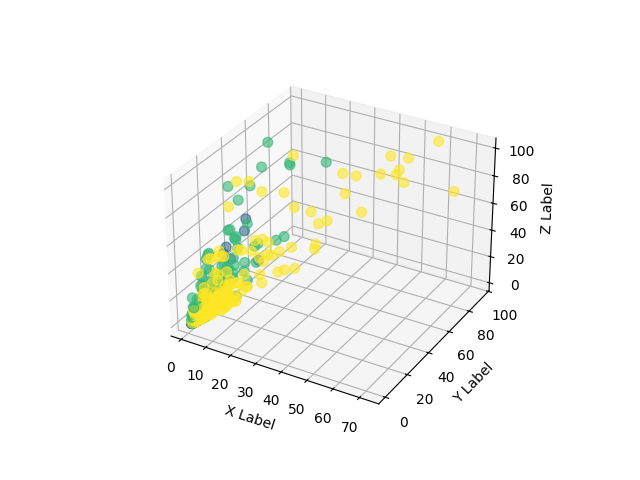
\includegraphics[scale=0.6]{3d_plot.png}
%\end{figure*}
On the other hand, the data themselves also yield interesting properties. If we consider a solution vector 
\begin{align*}
 s = \left( \dfrac{1}{C_1}, \dfrac{1}{C_2}, ..., \dfrac{1}{C_n} \right)
\end{align*}
For every two dimensions $ i \neq j$, the tank of the $i-$th plane is consumed before the $j-$th plane, or vice versa.
Formally speaking, either $C_1 < C_2$ or vice versa, and there is an equal amount of them, separated by the hyperplane 
$x_i - x_j = 0$. This separation is a valuable property and an interesting technique called \textbf{hyperplane arrangements} 
endeavors to research it.

\subsection{Formulation with Vasquez's Idea}
As an introduction, Vasquez's research \cite{vasquez2015airplane} on this problem was carefully studied 
in the early phase of this project. Later on, we re-dived into the paper for inspirations.
We also attempted to find a formulation based on his idea, but there was no success or flawed formulation. 
Hence, we do not bother to go into details. 

\section{Summary}
In this project, we reviewed a few pieces of literature on the airplane refueling problem and 
attempted to find a mathematical programming formulation for the problem. 
We gave a valid formulation, but it was not convex, and we were not able to solve it in polynomial time. 
This intractability is also evidence showing that this direction may not work.
\begin{enumerate}
    \item On the one hand, if we try to formulate this problem as a non-linear program problem, we end up 
 with a maximization problem over an unbounded convex feasible area or a bounded non-convex area. 
    \item On the other hand, if we try to find a linear programming formulation, in other words, a describing polytope, 
 it takes us exponential time to compute all facets in exchange for facets. 
\end{enumerate}
We can observe the first point from the first attempt on permutahedra, and we want to elaborate on the second point. 
Suppose we introduce one hyperplane for each constraining curve from \ref{eq:C}, we end up with polynomially many hyperplanes. 
However, we must compute each intersection, resulting in $n!$ many vertices and naturally exponential growth. 

Ultimately, we also want to point out other possibilities we have experimented with.
\begin{itemize}
    \item Extended formulation. As discussed in the previous section, more complex extended formulations may help solve this 
 problem. 
    \item Hyperplane Arrangements. Recall the results from data processing; we can witness a clear separation of vertices in the vector. 
 This property may be helpful for hyperplane arrangements, but there is no direct existing research from this aspect. 
    \item Deep Learning. Deep learning is always helpful in prediction. It may be helpful in predicting the number of facets or in the
 computation of our mathematical program. However, the interpretation of those results in formal mathematics remains a challenge. 
\end{itemize}

\bibliographystyle{plain}
\bibliography{../documentation/citations}

\end{document}
    